\section{Einführung in Design Patterns}

Entwurfsmuster oder auf Englisch `Design Patterns' sind bewährte Lösungsansätze für wiederkehrende Probleme, die bei der Konzeption der Software-Architektur oder während der Implementierung der Software
eingesetzt werden kann. Dabei dienen diese Entwurfsmuster als eine Art Blaupause, die es Software-Entwicklern ermöglicht, erprobte Lösungsstrategien für häufig auftretende Probleme in der Software-Entwicklung anzuwenden.
Durch den Einsatz von etablierten Entwurfsmustern können Software-Entwickler für die Software bei korrekter Anwendung unter anderem erhöhte Wartbarkeit, Wiederverwendbarkeit von Komponenten, Verständlichkeit und Skalierbarkeit ermöglichen das wiederum in qualitativ besserer Software resultiert.
Dabei sollte beachtet werden, dass Design Patterns als Vorlage zu betrachten sind. Je nach Einsatzgebiet muss die Anwendung des Entwurfsmusters evaluiert und für den konkreten Fall individualisiert werden.
Deshalb existiert keine universelle anwendbare Iteration eines Design Patterns, die unabhängig von Anwendungskontext eingesetzt werden kann. Dies resultiert in variierenden Anwendung von Entwurfsmustern abhängig von jeweiligem Einsatzgebiet.
Im weiteren Entwicklungszyklus der Software werden durch neue oder geänderte Anforderungen bereits eingesetzte Implementierungen von Entwurfsmustern modifiziert, entfernt oder neue werden hinzugefügt.
Währenddessen besteht die Gelegenheit, dass durch mangelnder Dokumentation oder anderer Gründe die Entscheidungen, weshalb Entwurfsmuster so eingesetzt sind wie es eingesetzt worden, verloren gehen.
Dadurch besteht die Gefahr, dass angewendete Design Patterns im weiteren Verlauf derer Entwicklung nicht mehr wiederzuerkennen sind. Aus diesem Grund ist die Etablierung eines Prozesses von Vorteil, das in der Lage ist,
Implementierungen von Entwurfsmustern aus einem Software-System zu extrahieren und dieses konkret benennen. Vor allem der Einsatz von Maschine Learning für die Klasszifierung ist hier vorteilhaft, wodurch das Potenzial besteht, vorher nicht gesehene Implementierung von Design Patterns zu erkennen.
% Durch solch einen Prozess können durch die Erkennung von eingesetzten Entwurfsmustern auf konkrete und verlorenen gegangene Design-Entscheidungen zurückgeschlossen werden, welche zukünftige Design-Entscheidungen für das Software-System beeinflussen können. 
Der Fokus dieser Arbeit besteht daran, solch ein Prozess zu etablieren, welches für ein gegebenes Set von Quellcode-Dateien mithilfe von Maschine Learning einem potenziellen Entwurfsmuster zuzuteilen.  

\pagebreak

\section{Untersuchungsfragen}

Das Ziel dieser Arbeit besteht aus der Etablierung eines Prozesses, womit durch Einsatz von Maschine Learning für ein Set von Quellcode-Dateien ein Design Pattern zuzuordnen.
Hierfür dienen eine Menge an Quelldateien als Eingabe für den Prozess und durch phasenweiser Transformationen und Bearbeitungen sollen ein möglichst passendes aus dem in Kontext dieser Arbeit betrachteten Entwurfsmusters zugeordnet werden.
Um solch ein Prozess zu entwickeln, werden in Kontext dieser Arbeit folgende Fragen beantwortet:

\begin{questions}
    \item\label{RQ1} Welche Design Patterns werden berücksichtigt?
    \item\label{RQ2} Was für ein Datensatz eignet sich für solch ein Prozess?
    \item\label{RQ3} Wonach wird exakt klassifiziert?
    \item\label{RQ4} Welche Merkmale, die aus Quellcode-Dateien extrahierbar sind, eignen sich für Klasszifierung durch Maschine Learning Modelle?  
    \item\label{RQ5} Welche Klassifizierer eignen sich?
    \item\label{RQ6} Wie wird eine Instanz eines Entwurfsmusters bestimmt?
\end{questions}


\section{Übersicht der Methodik}

In diesem Abschnitt wird erläutert, wie die in dieser Arbeit vorgeschlagene Methodik aufgebaut ist. 
Diese ist dabei in zwei Teile aufzuteilen.

\begin{figure}[h]
    \centering
    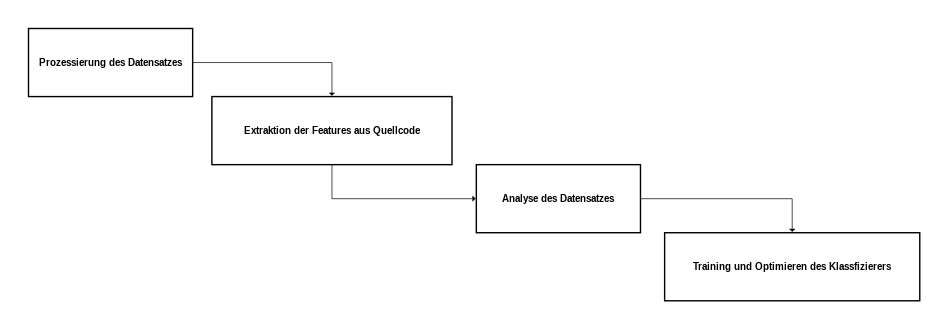
\includegraphics[scale=0.45]{figures/training_overview.png}
    \caption{Prozessabbildung des Trainings des Klassifizierers}
    \label{fig:training_process}
\end{figure}

Abbildung~\ref{fig:training_process} stellt die notwendigen Schritte dar, um einen Klassifizierer zu trainieren. Diese hat die Aufgabe,
Quellcodeentiäten eine Rolle im Kontext eines Entwurfsmusters zuzuordnen, das zu klassifizieren ist. Im ersten Schritt werden die notwendigen Informationen wie zugeordnetes Design Pattern und Rolle extrahiert und in einer CSV-Datei abgelegt. 
Diese CSV-Datei dient zusammen mit dem eigentlichen Quellcode als Eingabe in der Feature-Extraktion in Form von Codemetriken. Die Einträge aus der CSV-Datei werden dabei mit dem berechneten Codemetriken erweitert.
Darauffolgend wird eine explorative Datenanalyse durchgeführt, damit sich ein Überblick über die Datenpunkte geschafft wird. Anhand dieser Auswertung wird bestimmt, welche Entwurfsmuster und Rollen zu Klassifikation verfügbar.
Zum Schluss wird der verarbeitete Datensatz verwendet, um einen Klassifizierer zu trainieren. Der Trainingsschritt beinhaltet unter anderem die Optimierung des Modells durch Hyperparameter-Tuning und dessen Validation durch Kreuzvalidierung.
Die beste Iteration der Klassifizierers dient dabei als Grundlage bei der Bestimmung eines passenden Design Patterns.


\begin{figure}[h]
    \centering
    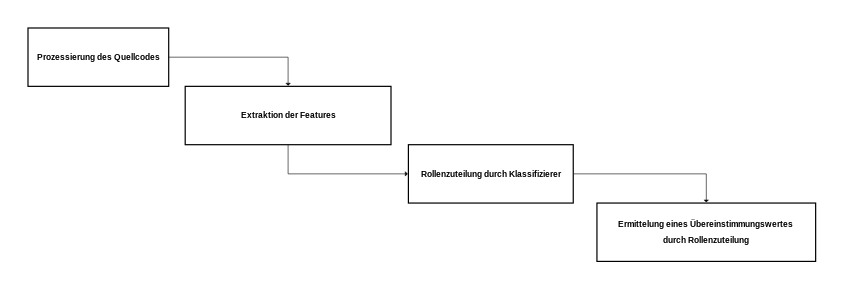
\includegraphics[scale=0.5]{figures/pattern_matching_overvierw.png}
    \caption{Prozessabbildung für Zuordnung von Entwurfsmustern}
    \label{fig:pattern_matching_overview}
\end{figure}

Die Abbildung~\ref{fig:pattern_matching_overview} beschreibt, wie auf Basis des vorher trainierten Klassifizierers ein Übereinstimmungswert ermittelt wird, der angibt,
welches Entwurfsmuster am ehesten zu den Quellcodeentiäten zuzuordnen ist. Wie im Trainingsprozess des Klassifizierers werden von den Quellcodeentiäten Codemetriken extrahiert.
Diese werden als Eingabe für den Klassifizierer verwendet. Durch die Bestimmung der Rollen wird für jedes betrachtete Design Pattern ein Übereinstimmungswert berechnet.
Das Design Pattern mit dem höchsten Übereinstimmungswert ist das Muster, welches am ehesten zu dem Set an Quellcodeentiäten passt.

